\section{Approach and Methodology}

\subsection{Overview}

The approach to this project remains aligned with the original proposal. The project is divided into four work packets based on the four research objectives. A brief overview of the proposed approach to each objective is provided below.

    {\color{secondary-text-color} \textit{NOTE: All objectives will broadly follow MLOps best practices, including version control, continuous integration, and automated testing. The project will be developed using Python, with a focus on open-source libraries and platforms like PyTorch and Kubernetes. An outline of the pipeline architecture that will serve as the backbone for this project is provided in \ref{fig:mlops}.}}

\begin{figure}[h]
    \centering
    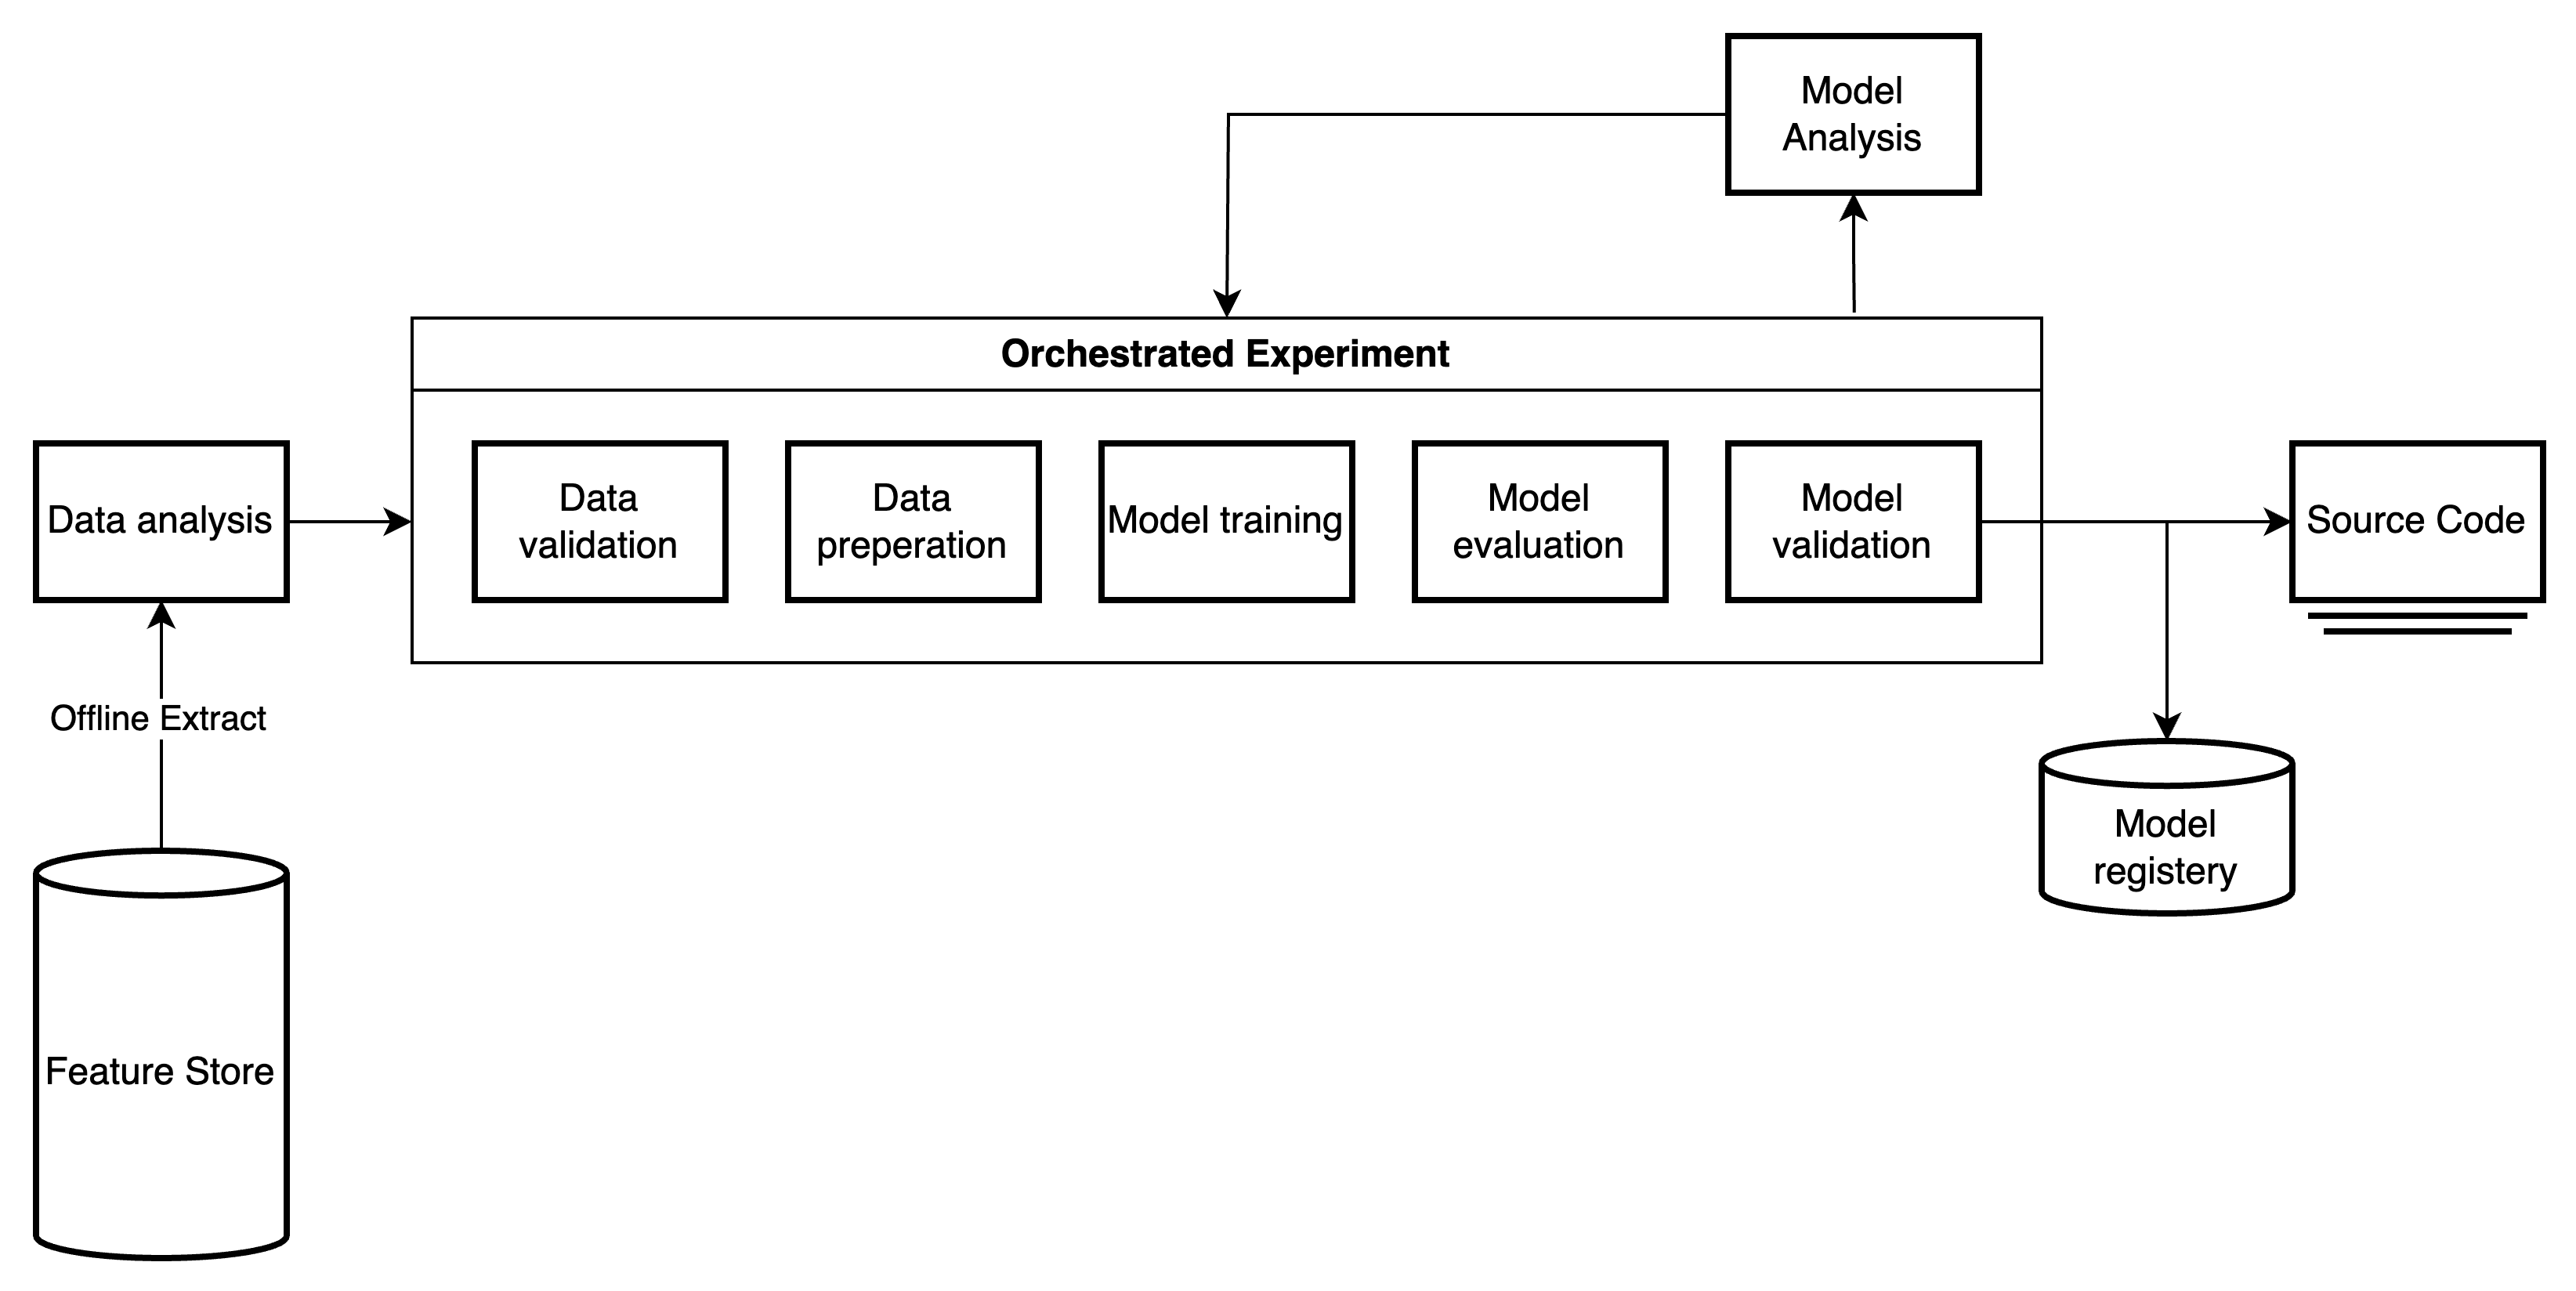
\includegraphics[scale=0.14]{figures/ml_ops.png}
    \caption{Proposed MLOps pipeline architecture for the project.}
    \label{fig:mlops}
\end{figure}

\subsection{Objective 1: Tools for Data Quality Assessment}

Developing tools that assess the quality of near real-time sensor data requires understanding the specific metrics and characteristics that define data quality. These metrics typically include accuracy, precision, timeliness, completeness, and reliability \cite{wangAccuracyWhatData1996}. The approach involves defining these quality parameters clearly, identifying the appropriate sensors and data sources, and then developing algorithms and tools to evaluate these aspects effectively.

The proposed approach begins with practical application case studies, such as pedestrian sensor data in railway stations to detect overcrowding. Data collection will use automated extraction tools for metrics like completeness and manual assessments for sensor-specific attributes such as object detection accuracy. To quantify DQ metrics like timeliness and accuracy, models such as those proposed by \cite{fizzaAgeDataAware2022}, who compute age of data to manage uncertainty during decision-making processes, will be used.

Comparative model evaluation will assess the impact of DQ metrics on prediction accuracy using statistical models like SARIMA and machine learning models including LSTMs and transformers. Metrics such as RMSE and R squared will be employed to evaluate model performance.

The methodology emphasises iterative testing and validation, ensuring that developed tools are robust and reliable. Initial findings will inform refinements, enhancing the tools’ applicability across different IoT contexts, thereby ensuring comprehensive and accurate assessments of sensor data quality.

\subsection{Objective 2: Spatio-Temporal Dependency Analysis}

This objective focuses on understanding the spatiotemporal dependencies within IoT data streams to determine sensor coverage adequacy. The methodology starts with an exploratory analysis to estimate expected data pattern lags, such as walking or driving times between sensors. This preliminary analysis sets the stage for training a deep learning model, like a graph neural network (GNN), to make spatiotemporal predictions.

An example case study involves a network of pedestrian sensors in a city centre. By analysing data counts and movement patterns, the network’s spatial distribution and reliability can be evaluated. The primary challenge is limited sensor distribution, which necessitates innovative pre-processing techniques. Methods like principal component analysis and Fourier analysis will decompose temporal signals, improving model performance \citep{kutzDynamicModeDecomposition2016}.

To assess spatiotemporal components, statistical methods such as spatial autocorrelation and dynamic time-warping \cite{froeseComparingTemporalGraphs2020}, alongside deep-learning approaches like hybrid GNNs, will be employed. Given the non-Euclidean nature of pedestrian networks, conventional CNNs are unsuitable \citep{klemmerAugmentingCorrelationStructures2019}. Instead, GNNs and GANs with local autocorrelation, as indicated by recent research, will be explored.

The model’s ability to predict spatiotemporal dependencies will be validated using performance metrics like RMSE and MAE. The goal is to establish a robust framework for analysing spatiotemporal dependencies, providing insights into the adequacy of sensor networks and informing future IoT deployments.

\subsection{Objective 3: ABM Assimilation}

The methodology for integrating agent-based model (ABM) outputs with real-time sensor data involves several key steps. First, a comprehensive review of existing surrogate modelling techniques will identify potential enhancements. The primary approach involves training deep learning models on ABM outputs, focusing on architectures capable of capturing high-dimensional, nonlinear relationships in urban dynamics.

Various deep learning architectures, such as hybrid GNN-LSTMs and GANs with local autocorrelation, will be explored. The ABM will be run offline to produce a spatiotemporally rich training set, which will train the surrogate model \citep{kieuRealtimePredictionsUsing2022}. This surrogate will then use real-time IoT sensor data to make predictions. For instance, pedestrian sensor data will be used to evaluate the surrogate’s ability to predict pedestrian counts.

The model’s performance will be evaluated on its ability to replicate ABM behaviours and make real-time predictions. The network of sensors will be split into training, testing, and validation sets. The surrogate’s predictions will be validated using metrics like RMSE, MAE, and R squared. The model’s ability to generalise across different sensor types and urban environments will also be assessed.

This methodology aims to create a computational bridge between ABMs and real-time IoT data, enabling efficient and accurate simulations of urban dynamics \citep{heppenstallFutureDevelopmentsGeographical2021}. The end goal is a robust surrogate model capable of real-time predictions, enhancing urban monitoring and decision-making processes.


\subsection{Objective 4: Approach Evaluation and Deployment Roadmap}

The final objective focuses on evaluating and scaling the developed methodologies using real-world case studies. The methodology involves collaboration with academic partners and stakeholders, such as Newcastle City Council and national data science institutes like DAFNI and the Alan Turing Institute. Initial stakeholder engagement will identify critical use cases, guiding the research focus.

A key aspect of this objective is a placement in a city with advanced IoT infrastructure, such as Singapore or Melbourne, providing a real-world testbed for the developed tools. The research will involve reflective evaluation to understand the scalability and generalisability of the methodologies. This includes testing the surrogate models on different ABMs and sensor networks, assessing performance across varying spatial and temporal resolutions.

Developing a roadmap for scalable deployment involves creating a translation framework to address challenges such as industry standards compliance and risk mitigation. This framework will demonstrate integration with existing digital infrastructure like DAFNI and explore improvements in computational efficiency, potentially through code optimisation.

Engagement with stakeholders will ensure the research addresses practical needs, facilitating the transition from pilot projects to deployable solutions. The objective aims to produce a pilot software library for real-time situational awareness and a roadmap for achieving higher technology readiness levels, paving the way for broader application and impact.
